%!TEX root = ../thesis.tex
%*******************************************************************************
%****************************** Fifth Chapter **********************************
%*******************************************************************************

\chapter{Experiments and Results}
\label{chapter6}

% **************************** Define Graphics Path **************************
\ifpdf
\graphicspath{{Chapter6/Figs/Raster/}{Chapter6/Figs/PDF/}{Chapter6/Figs/}}
\else
\graphicspath{{Chapter6/Figs/Vector/}{Chapter6/Figs/}}
\fi

\section{Learning the rates}

\section{Importance sampling}

\subsection{Single Particle on a Lattice}
\begin{equation}
	\partial_{t} \psi_{j}=\frac{1}{2}\left[\psi_{j+1}+\psi_{j-1}-2 \psi_{j}\right]+V_{j} \psi_{j}
\end{equation}

\begin{equation}
	\psi_{j}(t)=\underset{X \sim \mathrm{SRW} \text { with } X_{t}=j}{\mathbb{E}} \left[\exp \left(-\int_{0}^{t}  V\left(X_{\tau}, \tau\right) \mathrm{d} \tau \right) \psi_{X_{0}}(0)\right]
\end{equation}

\subsection{Transverse-field Ising model}
\label{sec:res-im}
\begin{figure}[h]
	\centering
	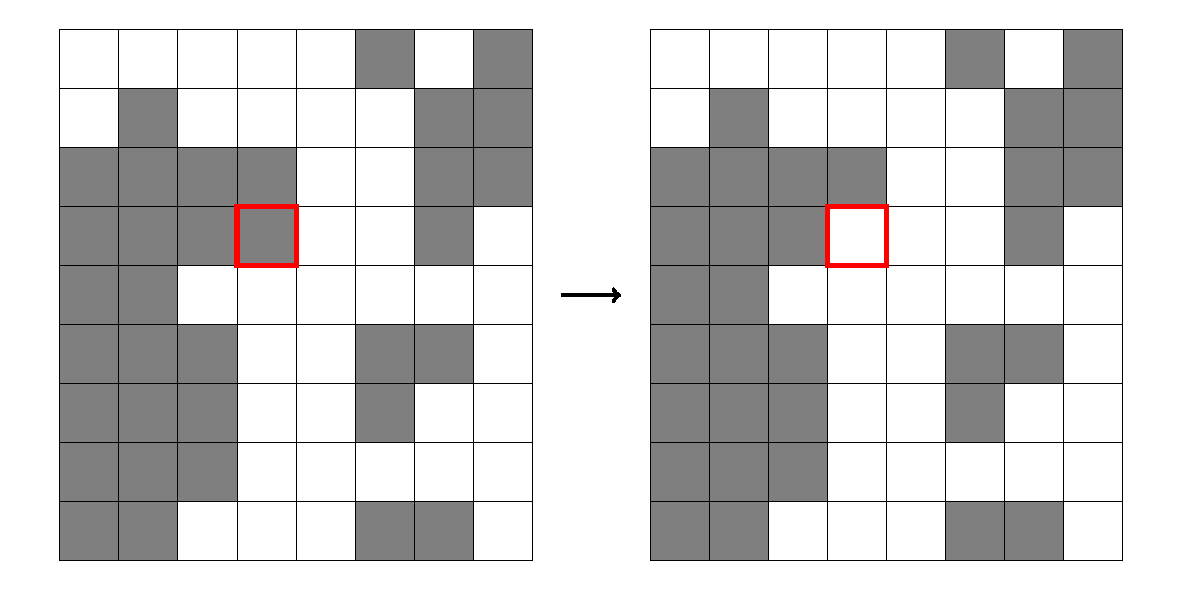
\includegraphics[width=\linewidth]{Chapter6/Figs/Vector/ising_passive}
	\caption[Ising passive process]{\textbf{Ising passive process}}	
	\label{fig:isingpassive}
\end{figure}

\subsection{Heisenberg model}
\label{sec:res-hm}
\begin{figure}[h]
	\centering
	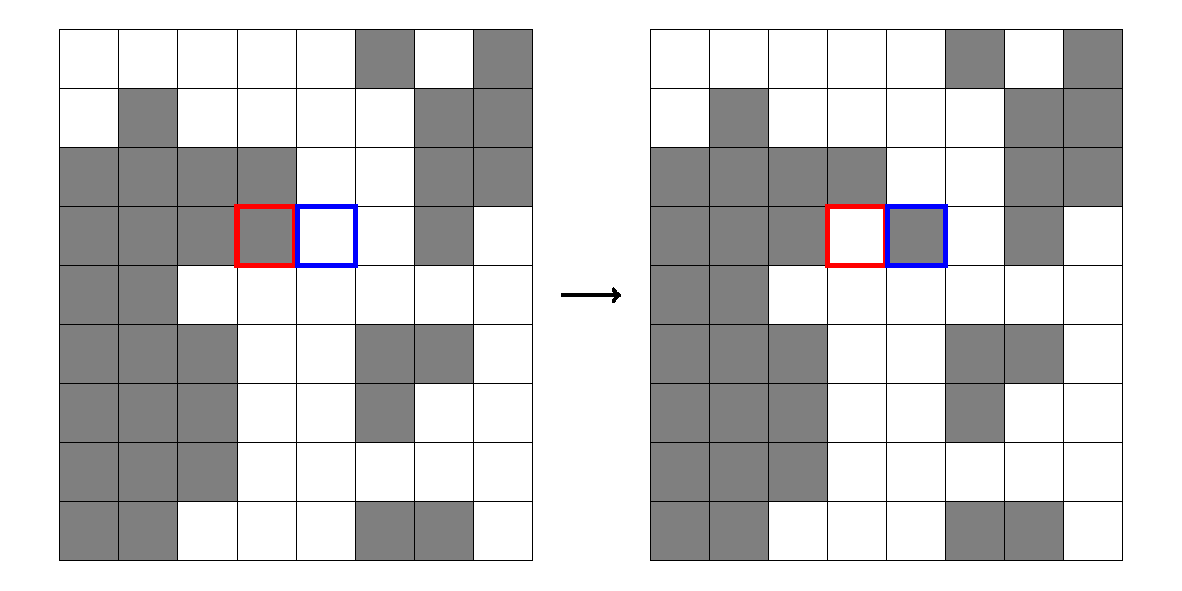
\includegraphics[width=\linewidth]{Chapter6/Figs/Vector/xy_passive}
	\caption[XY passive process]{\textbf{XY passive process}}
	\label{fig:xypassive}
\end{figure}

Heisenberg ferromagnet
\begin{equation}
	\hat H_{\mathrm{F}}=-\frac{1}{2} \sum_{j}\left[\hat{\sigma}_{j}^{x} \hat{\sigma}_{j+1}^{x}+\hat{\sigma}_{j}^{y} \hat{\sigma}_{j+1}^{y}+\hat{\sigma}_{j}^{z} \hat{\sigma}_{j+1}^{z}\right]
\end{equation}

The XY model.
\begin{equation}
	\begin{aligned} 
		\hat H_{X Y}=-\sum_{j}\left[\hat{\sigma}_{j}^{x} \hat{\sigma}_{j+1}^{x}+\hat{\sigma}_{j}^{y} \hat{\sigma}_{j+1}^{y}\right] &=H_{\mathrm{F}}+\frac{1}{2} \sum_{j} \hat{\sigma}_{j}^{z} \hat{\sigma}_{j+1}^{z} \\ 						&=-\mathcal{W}+\sum_{j}\left[n_{j}\left(1-n_{j+1}\right)+n_{j+1}\left(1-n_{j}\right)\right] 
	\end{aligned}
\end{equation}

\begin{equation}
	\psi_{s_{1: N}}(t)=\underset{\Sigma_{[0, t]} \sim \operatorname{SEP} \text{ with } \Sigma_{t}=s_{1: N}}{\mathbb{E}}
	\left[\exp \left(-\int_{0}^{t} d t^{\prime} \sum_{j}\left[n_{j}\left(1-n_{j+1}\right)+n_{j+1}\left(1-n_{j}\right)\right]\right) \psi_{\Sigma_{0}}(0)\right]
\end{equation}

\subsection{Bose-Hubbard model}
\label{sec:res-bhm}




